\ifdefined\inMainDoc\else
\documentclass[12pt,a4paper]{article}
% ================================================================
%  PRÉAMBULE COMMUN - ANNALES CORRIGÉES
%  Université de Kara - FaST - Licence Fondamentale MPC
%  Design optimisé impression noir et blanc
% ================================================================

% -- ENCODAGE & LANGUE --
\usepackage[utf8]{inputenc}
\usepackage[T1]{fontenc}
\usepackage[french]{babel}
\usepackage{lmodern}
\usepackage{microtype}

% -- MISE EN PAGE --
\usepackage[a4paper, top=2.8cm, bottom=2.5cm, left=2.5cm, right=2.5cm, headheight=14pt]{geometry}
\usepackage{setspace}
\setstretch{1.2}
\usepackage{parskip}
\setlength{\parindent}{1.2em}
\setlength{\parskip}{4pt}

% -- MATHS --
\usepackage{amsmath, amssymb, mathtools, amsthm}
\usepackage{mathrsfs}
\usepackage{dsfont}
\usepackage{bm}
\usepackage{cancel}
\usepackage{textcomp}
% Définition de \oiint (intégrale de surface fermée) sans package supplémentaire
\newcommand{\oiint}{\mathop{\iint\!\!\!\!\!\!\!\bigcirc}\limits}

% -- PHYSIQUE & CHIMIE --
\usepackage{physics}
\usepackage{siunitx}
% Lorsque physics est chargé, siunitx omet \qty. On le restaure ici :
\AtBeginDocument{\RenewCommandCopy\qty\SI}
\sisetup{locale = FR, detect-all, output-decimal-marker={,}}
% Commande de substitution pour les unités posant problème avec pdflatex
% (ohm, degreeCelsius, micro, angstrom, percent utilisent des caractères non-ASCII)
\newcommand{\qtyohm}[1]{\ensuremath{\num{#1}\,\Omega}}
\newcommand{\qtydegc}[1]{\ensuremath{\num{#1}\,{}^\circ\text{C}}}
\newcommand{\qtyangstrom}[1]{\ensuremath{\num{#1}\,\text{\AA}}}
\newcommand{\qtypercent}[1]{\ensuremath{\num{#1}\,\%}}
\newcommand{\qtyum}[1]{\ensuremath{\num{#1}\,\mu\text{m}}}
\usepackage[version=4]{mhchem}

% -- GRAPHISMES --
\usepackage{graphicx}
\usepackage{float}
\usepackage{caption}
\usepackage{subcaption}
\usepackage{wrapfig}
\usepackage{tikz}
\usetikzlibrary{calc, arrows.meta, patterns, shapes.geometric}
\usepackage{pgfplots}
\pgfplotsset{compat=1.18}

% -- TABLEAUX --
\usepackage{booktabs}
\usepackage{array}
\usepackage{tabularx}
\usepackage{multirow}

% -- LISTES --
\usepackage{enumitem}
\setlist[enumerate]{topsep=3pt, itemsep=2pt, parsep=0pt}
\setlist[itemize]{topsep=3pt, itemsep=2pt, parsep=0pt, label={.}}

% -- BOÎTES (noir et blanc) --
\usepackage{mdframed}
\usepackage{tcolorbox}
\tcbuselibrary{skins, breakable, theorems}

% Boîte EXERCICE : encadré avec filet épais, fond blanc
\newmdenv[
  linewidth=1.2pt,
  linecolor=black,
  roundcorner=3pt,
  skipabove=10pt,
  skipbelow=6pt,
  innertopmargin=8pt,
  innerbottommargin=8pt,
  innerleftmargin=10pt,
  innerrightmargin=10pt,
  backgroundcolor=white,
  frametitle={\bfseries\small Exercice},
  frametitlealignment=\raggedright,
  frametitleaboveskip=4pt,
  frametitlebelowskip=4pt,
]{boiteexercice}

% Boîte CORRIGÉ : fond gris très clair + filet fin
\newmdenv[
  linewidth=0.6pt,
  linecolor=black,
  leftline=true,
  rightline=false,
  topline=false,
  bottomline=false,
  linecolor=black,
  innerleftmargin=12pt,
  innerrightmargin=8pt,
  innertopmargin=6pt,
  innerbottommargin=6pt,
  backgroundcolor=gray!8,
  skipabove=4pt,
  skipbelow=8pt,
]{boitecorrige}

% Boîte RÉSUMÉ DE COURS : double encadré
\newmdenv[
  linewidth=0.8pt,
  linecolor=black,
  roundcorner=2pt,
  backgroundcolor=gray!12,
  innertopmargin=10pt,
  innerbottommargin=10pt,
  innerleftmargin=12pt,
  innerrightmargin=12pt,
  skipabove=12pt,
  skipbelow=8pt,
]{boiteresume}

% Boîte ATTENTION/REMARQUE : barre gauche épaisse
\newmdenv[
  leftline=true,
  rightline=false,
  topline=false,
  bottomline=false,
  linewidth=3pt,
  linecolor=black,
  backgroundcolor=gray!5,
  innerleftmargin=12pt,
  innerrightmargin=8pt,
  innertopmargin=5pt,
  innerbottommargin=5pt,
  skipabove=6pt,
  skipbelow=6pt,
]{boiteremarque}

% -- DIFFICULTÉ DES EXERCICES --
\newcommand{\facile}{$\star$}
\newcommand{\moyen}{$\star\!\star$}
\newcommand{\difficile}{$\star\!\star\!\star$}
\newcommand{\niveau}[1]{\hfill\textbf{#1}\hspace{2pt}}

% -- EN-TÊTES ET PIEDS DE PAGE --
\usepackage{fancyhdr}
\pagestyle{fancy}
\fancyhf{}
\renewcommand{\headrulewidth}{0.5pt}
\renewcommand{\footrulewidth}{0.3pt}

% -- HYPERLIENS --
\usepackage[hidelinks]{hyperref}
\hypersetup{
    colorlinks=false,
    pdftitle={Annale Corrigée - Licence MPC - Université de Kara}
}

% -- TITRES --
\usepackage{titlesec}
\titleformat{\section}{\Large\bfseries}{\thesection.}{0.8em}{}[\vspace{2pt}\hrule\vspace{4pt}]
\titleformat{\subsection}{\large\bfseries}{\thesubsection.}{0.7em}{}
\titleformat{\subsubsection}{\normalsize\bfseries}{\thesubsubsection.}{0.6em}{}

% -- THÉORÈMES --
\theoremstyle{definition}
\newtheorem{defn}{Définition}[section]
\newtheorem{prop}{Propriété}[section]
\newtheorem{thm}{Théorème}[section]
\newtheorem{corol}{Corollaire}[section]
\newtheorem{exemple}{Exemple}[section]

% -- COMMANDES MATHÉMATIQUES UTILES --
\newcommand{\vect}[1]{\overrightarrow{#1}}
\newcommand{\R}{\mathbb{R}}
\newcommand{\N}{\mathbb{N}}
\newcommand{\Z}{\mathbb{Z}}
\newcommand{\C}{\mathbb{C}}
\renewcommand{\d}{\mathrm{d}}
\newcommand{\deriv}[2]{\dfrac{\d #1}{\d #2}}
\newcommand{\dpart}[2]{\dfrac{\partial #1}{\partial #2}}
\newcommand{\rot}{\overrightarrow{\mathrm{rot}}\,}
\renewcommand{\div}{\mathrm{div}\,}
\renewcommand{\grad}{\overrightarrow{\mathrm{grad}}\,}
\newcommand{\e}{\mathrm{e}}
\newcommand{\ii}{\mathrm{i}}
\renewcommand{\Tr}{\mathrm{Tr}}

% Numérotation des équations par section
\numberwithin{equation}{section}

% -- RÉSULTATS ENCADRÉS --
\newcommand{\res}[1]{\[\boxed{#1}\]}

% -- REMARQUE INLINE --
\newcommand{\rmq}[1]{\begin{boiteremarque}\textbf{Remarque.} #1\end{boiteremarque}}

% -- MISE EN VALEUR DU RÉSULTAT FINAL --
\newcommand{\reponse}[1]{%
  \begin{center}
    \fbox{\begin{minipage}{0.92\textwidth}\centering #1\end{minipage}}
  \end{center}%
}


\lhead{\small\textit{Cristallographie - Licence 3}}
\rhead{\small\textit{FaST, Université de Kara}}
\cfoot{\thepage}

\begin{document}
\fi

\begin{center}
  {\LARGE\bfseries CRISTALLOGRAPHIE}\\[0.3cm]
  {\normalsize Licence 3 - Physique}\\[0.1cm]
  \rule{0.7\textwidth}{0.8pt}
\end{center}

\section*{Résumé du cours}

\begin{boiteresume}

\textbf{1. Réseaux de Bravais et mailles élémentaires.}
Un réseau de Bravais est un ensemble infini de points défini par les vecteurs de translation $\vec{T} = n_1\vec{a}+n_2\vec{b}+n_3\vec{c}$, $n_i\in\Z$. Il existe 14 réseaux de Bravais répartis en 7 systèmes cristallins. La maille élémentaire est le parallélépipède de base $(\vec{a},\vec{b},\vec{c})$ qui engendre le réseau par translation. La multiplicité (nombre d'atomes par maille) dépend du type de réseau : simple (1), centré CC (2), faces centrées CFC (4), base centrée (2).

\textbf{2. Indices de Miller.}
Un plan cristallographique $(hkl)$ est défini par ses intersections $a/h$, $b/k$, $c/l$ avec les axes. Une direction $[uvw]$ est le vecteur $u\vec{a}+v\vec{b}+w\vec{c}$. La famille de plans $\{hkl\}$ regroupe tous les plans équivalents par symétrie.

\textbf{3. Structures cristallines courantes.}
\begin{itemize}[nosep]
  \item Cubique simple (CS) : $z=1$, compacité $\pi/6 \approx 52\,\%$.
  \item Cubique centré (CC) : $z=2$, tangence selon la grande diagonale $4r=a\sqrt{3}$, compacité $\approx 68\,\%$.
  \item Cubique à faces centrées (CFC) : $z=4$, tangence sur la diagonale des faces $4r=a\sqrt{2}$, compacité $\approx 74\,\%$.
  \item Hexagonal compact (HC) : $z=2$, empilement ABAB, compacité $\approx 74\,\%$.
\end{itemize}

\textbf{4. Réseau réciproque.}
Les vecteurs de base réciproques sont $\vec{a}^* = \tfrac{\vec{b}\wedge\vec{c}}{V}$, etc., avec $V = \vec{a}\cdot(\vec{b}\wedge\vec{c})$. Pour un réseau orthorhombique ($\alpha=\beta=\gamma=90^\circ$), $a^*=1/a$, $b^*=1/b$, $c^*=1/c$. La distance réticulaire entre plans $(hkl)$ est $d_{hkl} = 1/|\vec{n}_{hkl}^*|$.

\textbf{5. Diffraction des rayons X : loi de Bragg.}
La diffraction a lieu selon la loi de Bragg : $2d_{hkl}\sin\theta = n\lambda$, où $d_{hkl}$ est la distance interréticulaire, $\theta$ l'angle de diffraction et $\lambda$ la longueur d'onde. Les rayons X sont diffractés de façon discontinue (pics de diffraction).

\textbf{6. Facteur de structure et facteur de forme.}
Le facteur de structure $F_{hkl} = \sum_j f_j\,\e^{2\pi\ii(hx_j+ky_j+lz_j)}$ détermine l'intensité des pics de diffraction. Les extinctions systématiques (réflexions interdites) sont liées à la symétrie du réseau.

\end{boiteresume}

\newpage
\subsection*{Exercice 1 - Vrai ou faux - notions fondamentales \niveau{\facile}}

\begin{boiteexercice}
\niveau{\facile}
Indiquer si chacune des affirmations suivantes est vraie ou fausse, en justifiant brièvement.

\begin{enumerate}
\item $(hkl)$ sont les longueurs découpées sur les axes par le plan noté $(hkl)$.
\item $[uvw]$ représente les coordonnées d'un atome dans la maille.
\item Le réseau réciproque est périodique et fini.
\item Un groupe ponctuel est plus symétrique qu'un groupe d'espace.
\item $4_2$ est un axe hélicoïdal.
\item P2/c est un groupe ponctuel.
\item L'axe $2$ est plus symétrique que l'axe $3$.
\item La maille simple pour la structure CFC est un rhomboèdre.
\item La direction $[110]$ dans la structure CFC est plus dense que la direction $[111]$ dans une structure CC.
\item Le cristal NaCl est composé de l'emboîtement de deux réseaux CC et CFC.
\item Les indices de Miller sont valables pour tous les systèmes cristallins.
\item L'empilement des couches dans la structure CFC est de type ABAB.
\item La maille triclinique possède un centre de symétrie.
\item La maille CFC contient une seule lacune octaédrique.
\item Les rayons X sont diffractés par un cristal de façon continue.
\item La structure cristalline est moins symétrique que le réseau cristallin.
\item Le réseau réciproque est périodique et infini.
\item $4_2$ est un axe de rotation direct.
\item 2,2,2,1 est un groupe ponctuel.
\item L'axe $3$ est plus symétrique que l'axe $2$.
\item La maille simple pour la structure CC est un rhomboèdre.
\item La direction $[110]$ dans la structure CC est plus dense que la direction $[111]$ dans une structure CFC.
\item Le plan $(10\bar{1}0)$ est moins dense que le plan $(0001)$ dans la structure hexagonale.
\item Le cristal NaCl est composé de l'emboîtement de deux réseaux CC.
\item L'empilement des couches dans la structure HC est de type ABAB.
\item La maille triclinique possède un plan de symétrie.
\item La densité électronique est périodique dans un cristal.
\item La structure diamant contient des lacunes tétraédriques.
\item Structure cristalline $-$ translation $=$ groupe ponctuel.
\item Les rayons X sont diffractés par un cristal de façon discontinue.
\item La structure cristalline est moins symétrique que le réseau cristallin.
\item La structure cubique CC est moins compacte que la structure cubique CFC.
\item La symétrie de translation existe dans une figure finie.
\item L'axe d'ordre $5$ existe dans une figure périodique infinie.
\item Les rayons X sont diffractés par un matériau amorphe.
\end{enumerate}
\end{boiteexercice}

\begin{boitecorrige}

\begin{enumerate}
\item \textbf{Faux.} $(hkl)$ sont les indices de Miller du plan, pas les longueurs découpées sur les axes.
\item \textbf{Faux.} $[uvw]$ représente une direction cristallographique, pas les coordonnées d'un atome.
\item \textbf{Faux.} Le réseau réciproque est périodique et \emph{infini}.
\item \textbf{Faux.} Un groupe d'espace est plus riche en symétrie car il inclut les translations.
\item \textbf{Vrai.} $4_2$ est bien un axe hélicoïdal d'ordre 4 (rotation de $90°$ combinée à une translation de $c/2$).
\item \textbf{Faux.} P2/c est un groupe d'espace (notation d'Hermann-Mauguin), pas un groupe ponctuel.
\item \textbf{Faux.} L'axe 3 est plus symétrique que l'axe 2 (ordre de symétrie plus élevé).
\item \textbf{Vrai.} La maille primitive de la structure CFC est un rhomboèdre d'angle $60°$.
\item \textbf{Vrai.} Dans CFC, $[110]$ est la direction de plus grande densité linéaire.
\item \textbf{Vrai.} NaCl est formé de deux réseaux CFC décalés de $a/2$, composés respectivement de Na$^+$ et Cl$^-$.
\item \textbf{Vrai.} Les indices de Miller s'appliquent à tous les systèmes cristallins (avec la convention à 4 indices pour l'hexagonal).
\item \textbf{Faux.} L'empilement CFC est de type ABCABC.
\item \textbf{Faux.} La maille triclinique n'a pas nécessairement de centre de symétrie (tout dépend du groupe d'espace).
\item \textbf{Faux.} La maille CFC contient 4 lacunes octaédriques (une par atome) et 8 lacunes tétraédriques.
\item \textbf{Faux.} Les rayons X sont diffractés de façon \emph{discontinue} (pics de diffraction aux angles de Bragg).
\item \textbf{Vrai.} La structure cristalline (réseau + motif) est en général moins symétrique que le réseau seul.
\item \textbf{Vrai.}
\item \textbf{Faux.} $4_2$ est un axe \emph{hélicoïdal}, pas un axe de rotation pure.
\item \textbf{Faux.} La notation 2,2,2,1 n'est pas une notation standard pour un groupe ponctuel.
\item \textbf{Vrai.}
\item \textbf{Faux.} La maille simple pour CC est un cube, pas un rhomboèdre.
\item \textbf{Faux.} La direction $[111]$ dans CFC est plus dense que $[110]$ dans CC.
\item \textbf{Vrai.} Le plan basal $(0001)$ est le plan le plus dense en hexagonal.
\item \textbf{Faux.} NaCl est formé de deux réseaux CFC imbriqués, pas CC.
\item \textbf{Vrai.} L'empilement HC est de type ABAB.
\item \textbf{Faux.} La maille triclinique ne possède pas nécessairement de plan de symétrie.
\item \textbf{Vrai.} La densité électronique $\rho(\vec{r})$ est une fonction périodique dans un cristal.
\item \textbf{Vrai.} La structure diamant comporte des sites tétraédriques partiellement occupés.
\item \textbf{Vrai.} Retirer les translations d'un groupe d'espace donne le groupe ponctuel associé.
\item \textbf{Vrai.} (Répétition de la question 15 avec la réponse correcte.)
\item \textbf{Vrai.} (Répétition de la question 16.)
\item \textbf{Vrai.} La compacité de CC ($68\,\%$) est inférieure à celle de CFC ($74\,\%$).
\item \textbf{Faux.} La symétrie de translation n'existe que dans une figure périodique infinie.
\item \textbf{Faux.} Un axe d'ordre 5 est incompatible avec la périodicité cristalline (théorème de restriction cristallographique).
\item \textbf{Faux.} Un matériau amorphe ne produit pas de pics de diffraction nets (halo diffus seulement).
\end{enumerate}

\textbf{Définitions essentielles.}

\textbf{Réseau cristallin :} Arrangement périodique et infini de points dans l'espace, représentant la périodicité translationnelle du cristal.

\textbf{Motif cristallin :} Arrangement d'atomes ou de molécules associé à chaque n\oe{}ud du réseau et qui se répète de façon identique.

\textbf{Structure cristalline :} Combinaison du réseau cristallin et du motif, décrivant l'arrangement complet des atomes dans le cristal.

\textbf{Maille cristalline :} Parallélépipède élémentaire qui, répété par translation dans les trois directions, reconstitue tout le cristal.

\textbf{Réseau réciproque :} Réseau mathématique dans l'espace de Fourier dont les n\oe{}uds correspondent aux vecteurs de diffraction possibles.

\textbf{Élément de symétrie :} Opération géométrique (rotation, réflexion, inversion, translation hélicoïdale) qui laisse le cristal globalement invariant.

\textbf{Groupe ponctuel :} Ensemble des opérations de symétrie qui laissent invariant au moins un point du cristal (rotations, réflexions, inversion).

\textbf{Groupe d'espace :} Ensemble complet des opérations de symétrie (y compris les translations) qui laissent le cristal invariant.

\end{boitecorrige}

\subsection*{Exercice 2 - Multiplicité des mailles \niveau{\facile}}

\begin{boiteexercice}
\niveau{\facile}
Calculer la multiplicité (nombre d'atomes par maille) pour :
\begin{enumerate}[label=\alph*)]
  \item le réseau cubique simple,
  \item le réseau cubique à faces centrées.
\end{enumerate}
\end{boiteexercice}

\begin{boitecorrige}
\textbf{a) Cubique simple.} Chaque sommet appartient à 8 mailles adjacentes :
\[
z = 8 \times \frac{1}{8} = 1 \text{ atome par maille.}
\]

\textbf{b) Cubique à faces centrées.} Sommets et centres des faces :
\[
z = 8 \times \frac{1}{8} + 6 \times \frac{1}{2} = 1 + 3 = 4 \text{ atomes par maille.}
\]
\end{boitecorrige}

\subsection*{Exercice 3 - Structure CFC : paramètre de maille et compacité \niveau{\moyen}}

\begin{boiteexercice}
\niveau{\moyen}
Pour la maille cubique à faces centrées :
\begin{enumerate}
  \item Calculer le nombre d'atomes $z$ par maille.
  \item Trouver la relation entre le rayon $r$ de l'atome et le paramètre de maille $a$.
  \item Calculer la compacité de cette structure.
\end{enumerate}
\end{boiteexercice}

\begin{boitecorrige}
\begin{enumerate}
\item D'après le résultat précédent, $z = 4$ atomes par maille.

\item Dans la structure CFC, les atomes sont en contact selon la diagonale d'une face. La diagonale de la face vaut $a\sqrt{2}$ et elle est égale à $4r$ :
\[
a\sqrt{2} = 4r \implies r = \frac{a\sqrt{2}}{4} = \frac{a}{2\sqrt{2}}.
\]

\begin{center}
\begin{tikzpicture}[scale=1.8, line join=round]
  % Arêtes visibles du cube CFC
  \pgfmathsetmacro{\a}{1.5}
  % Face avant
  \draw[thick] (0,0,0) -- (\a,0,0) -- (\a,\a,0) -- (0,\a,0) -- cycle;
  % Face droite
  \draw[thick] (\a,0,0) -- (\a,0,\a) -- (\a,\a,\a) -- (\a,\a,0);
  % Face haute
  \draw[thick] (0,\a,0) -- (0,\a,\a) -- (\a,\a,\a);
  % Arêtes arrière (en tirets)
  \draw[thick, dashed] (0,0,0) -- (0,0,\a) -- (\a,0,\a);
  \draw[thick, dashed] (0,0,\a) -- (0,\a,\a);
  % Atomes aux 8 sommets
  \foreach \x in {0,\a} \foreach \y in {0,\a} \foreach \z in {0,\a}
    \shade[ball color=blue!60] (\x,\y,\z) circle (0.18);
  % Atomes sur les 6 faces (centres)
  \shade[ball color=red!70] (\a/2,\a/2,0) circle (0.18);   % face avant
  \shade[ball color=red!70] (\a/2,\a/2,\a) circle (0.18);  % face arrière
  \shade[ball color=red!70] (\a/2,0,\a/2) circle (0.18);   % face bas
  \shade[ball color=red!70] (\a/2,\a,\a/2) circle (0.18);  % face haut
  \shade[ball color=red!70] (0,\a/2,\a/2) circle (0.18);   % face gauche
  \shade[ball color=red!70] (\a,\a/2,\a/2) circle (0.18);  % face droite
  % Diagonale de la face avant avec annotation
  \draw[red!80, thick, <->] (0,0,0) -- (\a,\a,0)
    node[midway, below right, font=\scriptsize] {$a\sqrt{2} = 4r$};
  % Paramètre a
  \draw[blue!70, <->] (0,-0.3,0) -- (\a,-0.3,0)
    node[midway, below, font=\scriptsize] {$a$};
\end{tikzpicture}
\captionof{figure}{\small Maille CFC : atomes de sommets (bleu) et de faces (rouge). La diagonale d'une face vaut $a\sqrt{2} = 4r$.}
\end{center}

\item La compacité est le rapport du volume occupé par les atomes sur le volume de la maille :
\[
C = \frac{z \cdot \frac{4}{3}\pi r^3}{a^3}
= \frac{4 \cdot \frac{4}{3}\pi\left(\frac{a}{2\sqrt{2}}\right)^3}{a^3}
= \frac{\frac{16\pi}{3}\cdot\frac{a^3}{16\sqrt{2}}}{a^3}
= \frac{\pi}{3\sqrt{2}} \approx 0{,}74 = 74\,\%.
\]
\end{enumerate}
\end{boitecorrige}

\subsection*{Exercice 4 - Polonium : compacité et masse volumique \niveau{\moyen}}

\begin{boiteexercice}
\niveau{\moyen}
Le polonium cristallise dans le système cubique simple de paramètre $a = 335{,}2\;\text{pm}$ et de masse molaire $M_\text{Po} = 209\;\text{g\,mol}^{-1}$.
\begin{enumerate}
  \item Calculer la compacité du polonium.
  \item Calculer la masse volumique du cristal.
\end{enumerate}
\end{boiteexercice}

\begin{boitecorrige}
\begin{enumerate}
\item Dans le cubique simple, les atomes sont tangents le long des arêtes : $a = 2r$, soit $r = a/2$. Avec $z=1$ :
\[
C = \frac{\frac{4}{3}\pi\left(\frac{a}{2}\right)^3}{a^3} = \frac{\pi}{6} \approx 0{,}52 = 52\,\%.
\]

\item
\[
\rho = \frac{z\cdot M_\text{Po}/N_A}{a^3}
= \frac{1 \times 209\times10^{-3}/6{,}022\times10^{23}}{(335{,}2\times10^{-12})^3}
\approx 9{,}22\times10^3\;\text{kg\,m}^{-3}.
\]
\end{enumerate}
\end{boitecorrige}

\subsection*{Exercice 5 - Dioxygène solide : nombre de molécules par maille \niveau{\facile}}

\begin{boiteexercice}
\niveau{\facile}
Le dioxygène solide cristallise dans un système cubique de paramètre $a = 683\;\text{pm}$ et de masse volumique $\rho = 1{,}32\;\text{kg\,m}^{-3}$.

Combien de molécules de $\text{O}_2$ la maille contient-elle ? (Donner : $M_{\text{O}_2} = 32\;\text{g\,mol}^{-1}$.)
\end{boiteexercice}

\begin{boitecorrige}
On écrit la masse volumique en fonction du nombre $N$ de molécules par maille :
\[
\rho = \frac{N\cdot M}{N_A\cdot a^3}
\implies N = \frac{\rho\cdot N_A\cdot a^3}{M}
= \frac{1{,}32 \times 6{,}022\times10^{23} \times (683\times10^{-12})^3}{32\times10^{-3}}
\approx 7{,}9 \approx 8.
\]
La maille contient \textbf{8 molécules} de $\text{O}_2$.
\end{boitecorrige}

\subsection*{Exercice 6 - Réseau réciproque \niveau{\moyen}}

\begin{boiteexercice}
\niveau{\moyen}
\begin{enumerate}
  \item Représenter l'allure du réseau réciproque d'un réseau orthorhombique ($\alpha=\beta=\gamma=90°$).
  \item Représenter l'allure du réseau réciproque d'un réseau monoclinique ($\alpha=\gamma=90°$, $\beta\neq90°$).
\end{enumerate}
\end{boiteexercice}

\begin{boitecorrige}
\begin{enumerate}
\item Pour un réseau orthorhombique, les vecteurs réciproques sont parallèles aux vecteurs directs et de longueurs $a^*=1/a$, $b^*=1/b$, $c^*=1/c$. Les angles du réseau réciproque sont $\alpha^*=\beta^*=\gamma^*=90°$ : le réseau réciproque est aussi orthorhombique.

\item Pour un réseau monoclinique (axe $b$ unique) : $b^*=1/b$ reste perpendiculaire au plan $(ac)$, mais $a^*$ et $c^*$ sont inclinés. On a :
\[
a^* = \frac{1}{a\sin\beta},\quad c^* = \frac{1}{c\sin\beta},\quad \gamma^* = 180°-\beta,\quad \alpha^*=\beta^*=90°.
\]
Le réseau réciproque est monoclinique avec l'angle $\gamma^* = 180°-\beta$.
\end{enumerate}
\end{boitecorrige}

\subsection*{Exercice 7 - Réseau réciproque orthorhombique et distance réticulaire \niveau{\moyen}}

\begin{boiteexercice}
\niveau{\moyen}
\begin{enumerate}
  \item Déterminer la base réciproque d'un réseau orthorhombique ($a\neq b\neq c$, $\alpha=\beta=\gamma=90°$).
  \item En déduire l'expression de la distance réticulaire $d_{hkl}$.
\end{enumerate}
\end{boiteexercice}

\begin{boitecorrige}
\begin{enumerate}
\item Comme $\beta=\gamma=90°$, $\vec{a}^*$ est parallèle à $\vec{a}$ et la condition $\vec{a}\cdot\vec{a}^*=1$ donne $a^*=1/a$. De même $b^*=1/b$ et $c^*=1/c$. Les angles du réseau réciproque valent tous $90°$.

\item Le vecteur du réseau réciproque est $\vec{n}_{hkl}^* = h\vec{a}^*+k\vec{b}^*+l\vec{c}^*$, de norme carrée :
\[
|\vec{n}_{hkl}^*|^2 = h^2a^{*2}+k^2b^{*2}+l^2c^{*2} = \frac{h^2}{a^2}+\frac{k^2}{b^2}+\frac{l^2}{c^2}.
\]
Puisque $d_{hkl}=1/|\vec{n}_{hkl}^*|$ :
\[
\boxed{d_{hkl} = \left(\frac{h^2}{a^2}+\frac{k^2}{b^2}+\frac{l^2}{c^2}\right)^{-1/2}.}
\]
\end{enumerate}
\end{boitecorrige}

\subsection*{Exercice 8 - Distance interréticulaire - maille orthorhombique \niveau{\facile}}

\begin{boiteexercice}
\niveau{\facile}
Calculer la distance interréticulaire $d_{hkl}$ pour une maille orthorhombique de paramètres $a=0{,}82\;\text{nm}$, $b=0{,}94\;\text{nm}$, $c=0{,}75\;\text{nm}$ pour :
\begin{enumerate}[label=\alph*)]
  \item les plans $(123)$,
  \item les plans $(246)$.
\end{enumerate}
\end{boiteexercice}

\begin{boitecorrige}
On applique la formule $d_{hkl} = \left(\dfrac{h^2}{a^2}+\dfrac{k^2}{b^2}+\dfrac{l^2}{c^2}\right)^{-1/2}$.

\textbf{a)}
\[
d_{123} = \left(\frac{1}{0{,}82^2}+\frac{4}{0{,}94^2}+\frac{9}{0{,}75^2}\right)^{-1/2} \approx 0{,}21\;\text{nm.}
\]

\textbf{b)}
\[
d_{246} = \left(\frac{4}{0{,}82^2}+\frac{16}{0{,}94^2}+\frac{36}{0{,}75^2}\right)^{-1/2} \approx 0{,}11\;\text{nm.}
\]
On remarque que $d_{246} = d_{123}/2$, conformément à la propriété $d_{nh,nk,nl} = d_{hkl}/n$.
\end{boitecorrige}

\subsection*{Exercice 9 - Réseau réciproque de l'indium \niveau{\moyen}}

\begin{boiteexercice}
\niveau{\moyen}
L'indium cristallise à température ambiante dans un réseau tétragonal simple de paramètres $a=3{,}25\;\text{\AA}$ et $c=4{,}95\;\text{\AA}$.
\begin{enumerate}
  \item Déterminer son réseau réciproque.
  \item Calculer les volumes $V$ (maille directe) et $V^*$ (maille réciproque), puis le produit $V\times V^*$.
\end{enumerate}
\end{boiteexercice}

\begin{boitecorrige}
\begin{enumerate}
\item Pour un réseau tétragonal simple, $a=b\neq c$ et $\alpha=\beta=\gamma=90°$. Le réseau réciproque vérifie alors $a^*=b^*=1/a$, $c^*=1/c$ et $\alpha^*=\beta^*=\gamma^*=90°$. Le réseau réciproque est donc aussi \textbf{tétragonal primitif}.

\item
\begin{align*}
V &= a^2c = (3{,}25)^2\times 4{,}95 = 52{,}3\;\text{\AA}^3\\
V^* &= a^{*2}c^* = \frac{1}{a^2c} = \frac{1}{52{,}3} \approx 1{,}91\times10^{-2}\;\text{\AA}^{-3}
\end{align*}
Donc $V\times V^* = 1$, résultat général valable pour tout réseau :
le volume de la maille réciproque est l'inverse du volume de la maille directe.
\end{enumerate}
\end{boitecorrige}

\subsection*{Exercice 10 - Symétrie d'un cube peint \niveau{\moyen}}

\begin{boiteexercice}
\niveau{\moyen}
On considère un cube dont les faces sont peintes de couleurs différentes de sorte que la seule symétrie rotationnelle préservée soit l'axe $4$ passant par le centre de chaque paire de faces opposées (un seul axe $4$ unique), l'axe $3$ passant par les sommets et un axe $2$.
\begin{enumerate}
  \item Déterminer les éléments de symétrie de ce cube.
  \item À quel système cristallin appartient-il ?
  \item Donner la notation d'Hermann-Mauguin.
\end{enumerate}
\end{boiteexercice}

\begin{boitecorrige}
\begin{enumerate}
\item Les éléments de symétrie sont : un axe d'ordre 4 (selon une paire de faces opposées), quatre axes d'ordre 3 (diagonales principales du cube), six axes d'ordre 2 (centres des arêtes). Les peintures éliminent les plans de symétrie et le centre d'inversion.

\item Le système est \textbf{cubique}, car la présence d'au moins deux axes d'ordre 4 (ici un axe propre, caractéristique du cubique) et d'axes d'ordre 3 est la signature du système cubique.

\item Notation d'Hermann-Mauguin : $\mathbf{432}$, indiquant un axe principal d'ordre 4, des axes secondaires d'ordre 3 et des axes d'ordre 2.
\end{enumerate}
\end{boitecorrige}

\subsection*{Exercice 11 - Opérations de symétrie et groupes ponctuels \niveau{\difficile}}

\begin{boiteexercice}
\niveau{\difficile}
\begin{enumerate}
  \item Montrer qu'un axe $\bar{2}$ est équivalent à un plan miroir.
  \item Montrer qu'un axe $\bar{6}$ est équivalent à un axe $3$ perpendiculaire à un miroir.
\end{enumerate}
\end{boiteexercice}

\begin{boitecorrige}
\begin{enumerate}
\item L'axe $\bar{2}$ est une rotation-inversion d'ordre 2 : on effectue une rotation de $180°$ suivie d'une inversion par rapport au point fixe. Soit un point $M_1$. La rotation de $180°$ le porte en $M_2$ (point diamétralement opposé dans le plan perpendiculaire à l'axe), puis l'inversion porte $M_2$ en $M_3$. On constate que la transformation $M_1\to M_3$ est exactement une réflexion par rapport au plan perpendiculaire à l'axe : $\bar{2} \equiv m$.

\item L'axe $\bar{6}$ effectue une rotation de $60°$ suivie d'une inversion. En appliquant l'opération à un ensemble de points, on vérifie que les orbites générées sont identiques à celles produites par un axe 3 (rotation de $120°$) combiné avec un miroir perpendiculaire à cet axe : $\bar{6} \equiv 3\perp m$.
\end{enumerate}
\end{boitecorrige}

\subsection*{Exercice 12 - Rayons X : production et caractéristiques \niveau{\moyen}}

\begin{boiteexercice}
\niveau{\moyen}
Un tube à rayons X est équipé d'une anode et produit un faisceau de haute énergie.
\begin{enumerate}
  \item Pour une anode de cuivre (électrons à $40\;\text{keV}$) : donner les séries de raies émises.
  \item Calculer la transmission de la fenêtre en béryllium ($e=0{,}5\;\text{mm}$, $l_\text{abs}=5{,}371\;\text{mm}$ à $8050\;\text{eV}$) pour la raie $\text{K}\alpha$ du Cu.
  \item Pour une anode de tungstène (mêmes électrons à $40\;\text{keV}$) : donner les séries de raies accessibles.
\end{enumerate}
\end{boiteexercice}

\begin{boitecorrige}
\begin{enumerate}
\item Les électrons à $40\;\text{keV}$ ont une énergie supérieure à toutes les énergies de liaison des électrons du cuivre (énergie de la couche K du Cu : environ $8{,}98\;\text{keV}$). Toutes les couches peuvent être ionisées, donc les séries K$\alpha_1$, K$\alpha_2$, K$\beta$, L$\alpha$, L$\beta$ sont émises. La longueur d'onde se calcule par $\lambda\;[\text{nm}] = 1239{,}84\,/\,E\;[\text{eV}]$.

\item La loi d'atténuation donne la transmission :
\[
T = \e^{-e/l_\text{abs}} = \e^{-0{,}5/5{,}371} \approx 0{,}91 = 91\,\%.
\]

\item L'énergie de liaison de la couche K du tungstène est d'environ $69{,}5\;\text{keV}$, soit supérieure à $40\;\text{keV}$. Les raies K ne peuvent pas être émises. Seules les raies des couches L (et M) sont accessibles : L$\alpha_1$, L$\alpha_2$, L$\beta_1$, L$\beta_2$, L$\gamma$, M$\alpha$.
\end{enumerate}
\end{boitecorrige}

\subsection*{Exercice 13 - Tube émetteur de rayons X : calculs énergétiques \niveau{\moyen}}

\begin{boiteexercice}
\niveau{\moyen}
Dans un tube à rayons X, les électrons sont accélérés sous une tension $U = 60\;\text{kV}$. Données : masse de l'électron $m_e = 9{,}1\times10^{-31}\;\text{kg}$, $h = 6{,}62\times10^{-34}\;\text{J\,s}$, $e = 1{,}6\times10^{-19}\;\text{C}$.
\begin{enumerate}
  \item Calculer l'énergie cinétique acquise (en J et en keV) et la vitesse des électrons.
  \item Calculer la fréquence maximale du photon émis et la longueur d'onde correspondante.
  \item Pour une anode de tungstène ($Z=74$) et un rendement de $2\,\%$, calculer la constante $k$ du tube ($R = kZV$, avec $R$ le rendement, $V$ la tension).
  \item En déduire la puissance du rayonnement pour un courant anodique $I = 20\;\text{mA}$.
\end{enumerate}
\end{boiteexercice}

\begin{boitecorrige}
\begin{enumerate}
\item L'énergie cinétique est $E_c = eU = 1{,}6\times10^{-19}\times60\times10^3 = 9{,}6\times10^{-15}\;\text{J} = 60\;\text{keV}$.

Vitesse :
\[
v = \sqrt{\frac{2E_c}{m_e}} = \sqrt{\frac{2\times9{,}6\times10^{-15}}{9{,}1\times10^{-31}}} \approx 1{,}45\times10^8\;\text{m\,s}^{-1}.
\]

\item Fréquence maximale (toute l'énergie cinétique convertie en un seul photon) :
\[
\nu_\text{max} = \frac{E_c}{h} = \frac{9{,}6\times10^{-15}}{6{,}62\times10^{-34}} \approx 1{,}45\times10^{19}\;\text{Hz}.
\]
Longueur d'onde minimale :
\[
\lambda_\text{min} = \frac{c}{\nu_\text{max}} = \frac{3\times10^8}{1{,}45\times10^{19}} \approx 20{,}7\;\text{pm.}
\]

\item La constante $k$ vaut :
\[
k = \frac{R}{ZV} = \frac{0{,}02}{74\times60\times10^3} \approx 4{,}50\times10^{-9}.
\]

\item Puissance du rayonnement :
\[
P = kIZV^2 = 4{,}50\times10^{-9}\times20\times10^{-3}\times74\times(60\times10^3)^2 \approx 24\;\text{W.}
\]
\end{enumerate}
\end{boitecorrige}


\newpage
\section{Exercices supplémentaires de cristallographie}

\subsection*{Exercice 14 - Réseau cubique centré (CC) \niveau{\moyen}}

\begin{boiteexercice}
Pour une structure cubique centrée (CC) :
\begin{enumerate}
  \item Calculer le nombre d'atomes par maille.
  \item Trouver la relation entre le rayon atomique $r$ et le paramètre de maille $a$.
  \item Calculer la compacité.
  \item Le fer $\alpha$ cristallise en CC avec $a = 286{,}5\;\text{pm}$ et $M_{Fe} = 55{,}85\;\text{g\,mol}^{-1}$. Calculer la masse volumique.
\end{enumerate}
\end{boiteexercice}

\begin{boitecorrige}
\textbf{1.} Multiplicité : $8 \times \frac{1}{8} + 1 = 2$ atomes par maille.

\textbf{2.} Les atomes sont tangents le long de la grande diagonale du cube :
\[
4r = a\sqrt{3} \implies r = \frac{a\sqrt{3}}{4}
\]

\textbf{3.} Compacité :
\[
C = \frac{2 \times \frac{4}{3}\pi r^3}{a^3} = \frac{2 \times \frac{4}{3}\pi\left(\frac{a\sqrt{3}}{4}\right)^3}{a^3} = \frac{\pi\sqrt{3}}{8} \approx 0{,}68 = 68\,\%
\]

\textbf{4.} Masse volumique du fer $\alpha$ :
\[
\rho = \frac{z \cdot M_{Fe}}{N_A \cdot a^3} = \frac{2 \times 55{,}85 \times 10^{-3}}{6{,}022\times10^{23} \times (286{,}5\times10^{-12})^3} \approx 7875\;\text{kg\,m}^{-3}
\]
\end{boitecorrige}

\clearpage
\subsection*{Exercice 15 - Loi de Bragg et diffraction \niveau{\moyen}}

\begin{boiteexercice}
On fait diffracter des rayons X de longueur d'onde $\lambda = 154\;\text{pm}$ sur un cristal de nickel (CFC, $a = 352\;\text{pm}$).
\begin{enumerate}
  \item Calculer la distance interréticulaire $d_{111}$, $d_{110}$ et $d_{100}$.
  \item Calculer les angles de Bragg pour les plans $(111)$, $(200)$ et $(220)$ à l'ordre 1.
  \item Indiquer les extinctions systématiques dans un réseau CFC.
\end{enumerate}
\end{boiteexercice}

\begin{boitecorrige}
\textbf{1.} Pour un réseau cubique : $d_{hkl} = \dfrac{a}{\sqrt{h^2+k^2+l^2}}$.
\[
d_{111} = \frac{352}{\sqrt{3}} \approx 203{,}3\;\text{pm}, \quad d_{110} = \frac{352}{\sqrt{2}} \approx 248{,}9\;\text{pm}, \quad d_{100} = 352\;\text{pm}
\]

\textbf{2.} Loi de Bragg ($n=1$) : $2d\sin\theta = \lambda$, soit $\sin\theta = \dfrac{\lambda}{2d}$.

\begin{align*}
\theta_{111} &= \arcsin\!\left(\frac{154}{2\times203{,}3}\right) \approx 22{,}2^\circ \\
\theta_{200} &= \arcsin\!\left(\frac{154}{2\times176}\right) \approx 25{,}9^\circ \\
\theta_{220} &= \arcsin\!\left(\frac{154}{2\times124{,}5}\right) \approx 38{,}2^\circ
\end{align*}

\textbf{3.} Dans un réseau CFC, les extinctions systématiques ont lieu quand les indices $h$, $k$, $l$ sont mixtes (certains pairs et certains impairs). La réflexion est permise seulement si $h$, $k$, $l$ sont tous pairs ou tous impairs. Les plans $(100)$, $(110)$, $(210)$ sont interdits ; les plans $(111)$, $(200)$, $(220)$, $(311)$ sont permis.
\end{boitecorrige}

\subsection*{Exercice 16 - Structure NaCl et facteur de structure \niveau{\difficile}}

\begin{boiteexercice}
La structure NaCl est constituée de deux réseaux CFC imbriqués (Na$^+$ et Cl$^-$) décalés de $a/2$ selon un axe.
\begin{enumerate}
  \item Calculer le nombre d'ions Na$^+$ et Cl$^-$ par maille.
  \item Écrire les positions fractionnaires des ions.
  \item Calculer le facteur de structure $F_{hkl}$ pour NaCl. Identifier les conditions d'extinction.
  \item Le paramètre de maille de NaCl est $a = 562\;\text{pm}$, $M_{Na} = 23\;\text{g\,mol}^{-1}$, $M_{Cl} = 35{,}5\;\text{g\,mol}^{-1}$. Calculer la masse volumique.
\end{enumerate}
\end{boiteexercice}

\begin{boitecorrige}
\textbf{1.} Multiplicité de Na$^+$ : $12\times\frac{1}{4} + 1 = 4$ ions. Multiplicité de Cl$^-$ : $8\times\frac{1}{8} + 6\times\frac{1}{2} = 4$ ions. Total : 4 motifs NaCl.

\textbf{2.} Positions de Na$^+$ : $(0,0,0)$, $(\frac{1}{2},\frac{1}{2},0)$, $(\frac{1}{2},0,\frac{1}{2})$, $(0,\frac{1}{2},\frac{1}{2})$.

Positions de Cl$^-$ : $(\frac{1}{2},0,0)$, $(0,\frac{1}{2},0)$, $(0,0,\frac{1}{2})$, $(\frac{1}{2},\frac{1}{2},\frac{1}{2})$.

\textbf{3.} Le facteur de structure :
\[
F_{hkl} = f_{Na}\sum_{Na}\e^{2\pi\ii(hx_j+ky_j+lz_j)} + f_{Cl}\sum_{Cl}\e^{2\pi\ii(hx_j+ky_j+lz_j)}
\]
\[
= (f_{Na} + f_{Cl}\e^{\ii\pi(h+k+l)})\underbrace{(1+\e^{\ii\pi(h+k)}+\e^{\ii\pi(h+l)}+\e^{\ii\pi(k+l)})}_{\text{facteur CFC}}
\]

Le facteur CFC est nul si $h$, $k$, $l$ sont mixtes. Pour indices tous de même parité :
\begin{itemize}[nosep]
  \item Si $h+k+l$ pair : $F_{hkl} = 4(f_{Na} + f_{Cl})$
  \item Si $h+k+l$ impair : $F_{hkl} = 4(f_{Na} - f_{Cl})$
\end{itemize}

\textbf{4.} Masse volumique :
\[
\rho = \frac{4(M_{Na}+M_{Cl})}{N_A\cdot a^3} = \frac{4\times58{,}5\times10^{-3}}{6{,}022\times10^{23}\times(562\times10^{-12})^3} \approx 2163\;\text{kg\,m}^{-3}
\]
\end{boitecorrige}

\subsection*{Exercice 17 - Structure hexagonale compacte (HC) \niveau{\moyen}}

\begin{boiteexercice}
Dans la structure hexagonale compacte (HC) :
\begin{enumerate}
  \item Calculer le nombre d'atomes par maille.
  \item Trouver le rapport $c/a$ idéal.
  \item Calculer la compacité.
  \item Comparer avec la structure CFC.
\end{enumerate}
\end{boiteexercice}

\begin{boitecorrige}
\textbf{1.} La maille HC contient : 2 atomes (1 dans la maille + fractions des sommets et des faces basales) : $z = 2$.

\textbf{2.} Dans HC, les sphères de rayon $r$ sont tangentes. L'empilement ABAB impose :
\[
\frac{c}{a} = \sqrt{\frac{8}{3}} \approx 1{,}633
\]

\textbf{3.} Volume de la maille hexagonale : $V = \frac{\sqrt{3}}{2}a^2 c$. Relation $a = 2r$ :
\[
C = \frac{2\times\frac{4}{3}\pi r^3}{\frac{\sqrt{3}}{2}a^2 c} = \frac{\pi}{3\sqrt{2}} \approx 0{,}74 = 74\,\%
\]

\textbf{4.} La compacité de HC ($\approx74\,\%$) est identique à celle de CFC ($\approx74\,\%$). Les deux structures sont des empilements compacts de sphères dures, différant seulement dans la séquence d'empilement : ABCABC pour CFC et ABAB pour HC.

\begin{center}
\begin{tikzpicture}[scale=0.72]
  % ---- HC (ABAB) ----
  \node[font=\bfseries\small] at (1.8, 7.2) {HC : empilement ABAB};
  % Couche A (bas)
  \foreach \x in {0,1,2,3}
    \shade[ball color=blue!60] (\x*0.9, 0) circle (0.38);
  \node[right, font=\scriptsize] at (3.7, 0) {A};
  % Couche B
  \foreach \x in {0,1,2}
    \shade[ball color=red!60] (\x*0.9+0.45, 0.78) circle (0.38);
  \node[right, font=\scriptsize] at (3.7, 0.78) {B};
  % Couche A
  \foreach \x in {0,1,2,3}
    \shade[ball color=blue!60] (\x*0.9, 1.56) circle (0.38);
  \node[right, font=\scriptsize] at (3.7, 1.56) {A};
  % Couche B
  \foreach \x in {0,1,2}
    \shade[ball color=red!60] (\x*0.9+0.45, 2.34) circle (0.38);
  \node[right, font=\scriptsize] at (3.7, 2.34) {B};
  % Couche A
  \foreach \x in {0,1,2,3}
    \shade[ball color=blue!60] (\x*0.9, 3.12) circle (0.38);
  \node[right, font=\scriptsize] at (3.7, 3.12) {A};

  % ---- CFC (ABCABC) ----
  \node[font=\bfseries\small] at (9.0, 7.2) {CFC : empilement ABCABC};
  % Couche A (bas)
  \foreach \x in {0,1,2,3}
    \shade[ball color=blue!60] (\x*0.9+5.5, 0) circle (0.38);
  \node[right, font=\scriptsize] at (9.7, 0) {A};
  % Couche B
  \foreach \x in {0,1,2}
    \shade[ball color=red!60] (\x*0.9+5.95, 0.78) circle (0.38);
  \node[right, font=\scriptsize] at (9.7, 0.78) {B};
  % Couche C
  \foreach \x in {0,1,2}
    \shade[ball color=green!60!black] (\x*0.9+6.2, 1.56) circle (0.38);
  \node[right, font=\scriptsize] at (9.7, 1.56) {C};
  % Couche A
  \foreach \x in {0,1,2,3}
    \shade[ball color=blue!60] (\x*0.9+5.5, 2.34) circle (0.38);
  \node[right, font=\scriptsize] at (9.7, 2.34) {A};
  % Couche B
  \foreach \x in {0,1,2}
    \shade[ball color=red!60] (\x*0.9+5.95, 3.12) circle (0.38);
  \node[right, font=\scriptsize] at (9.7, 3.12) {B};

  % Séparateur
  \draw[gray, dashed] (4.8, -0.5) -- (4.8, 7.0);
\end{tikzpicture}
\captionof{figure}{\small Comparaison des empilements compacts : ABAB (structure HC, à gauche) et ABCABC (structure CFC, à droite). Les couleurs distinguent les positions A, B et C des couches atomiques.}
\end{center}
\end{boitecorrige}

\subsection*{Exercice 18 - Réseau réciproque et condition de Laue \niveau{\difficile}}

\begin{boiteexercice}
Considérer un réseau cubique simple de paramètre $a$.
\begin{enumerate}
  \item Calculer les vecteurs de base du réseau réciproque.
  \item Écrire la condition de Laue pour la diffraction.
  \item Montrer que la condition de Laue est équivalente à la loi de Bragg.
  \item Pour $\lambda = 150\;\text{pm}$ et $a = 400\;\text{pm}$, quelles familles de plans $(hkl)$ peuvent diffracter ?
\end{enumerate}
\end{boiteexercice}

\begin{boitecorrige}
\textbf{1.} Pour un réseau cubique ($\vec{a} = a\hat{x}$, $\vec{b} = a\hat{y}$, $\vec{c} = a\hat{z}$) :
\[
\vec{a}^* = \frac{1}{a}\hat{x}, \quad \vec{b}^* = \frac{1}{a}\hat{y}, \quad \vec{c}^* = \frac{1}{a}\hat{z}
\]
Le réseau réciproque est aussi cubique de paramètre $1/a$.

\textbf{2.} La condition de Laue : le vecteur de diffusion $\vec{Q} = \vec{k}_f - \vec{k}_i$ doit être un vecteur du réseau réciproque :
\[
\vec{Q} = h\vec{a}^* + k\vec{b}^* + l\vec{c}^* = \vec{G}_{hkl}
\]

\textbf{3.} Pour une diffusion élastique ($|\vec{k}_f| = |\vec{k}_i| = 1/\lambda$), on a $|\vec{Q}| = 2\sin\theta/\lambda$. Le module du vecteur réciproque est $|\vec{G}_{hkl}| = 1/d_{hkl}$. L'égalité donne :
\[
\frac{2\sin\theta}{\lambda} = \frac{1}{d_{hkl}} \implies 2d_{hkl}\sin\theta = \lambda
\]
C'est bien la loi de Bragg.

\textbf{4.} La condition est $2d_{hkl}\sin\theta = \lambda$ avec $\sin\theta \leq 1$, soit $d_{hkl} \geq \lambda/2 = 75\;\text{pm}$.
\[
d_{hkl} = \frac{400}{\sqrt{h^2+k^2+l^2}} \geq 75 \implies h^2+k^2+l^2 \leq \left(\frac{400}{75}\right)^2 \approx 28{,}4
\]
Les familles accessibles sont : $(100)$, $(110)$, $(111)$, $(200)$, $(210)$, $(211)$, $(220)$, $(300)$, $(221)$, $(310)$, $(311)$, $(222)$, $(320)$, $(321)$.
\end{boitecorrige}


\subsection*{Exercice 19 - Loi de Bragg et diffraction X \niveau{\moyen}}

\begin{boiteexercice}
Un cristal cubique face centrée (CFC) d'aluminium ($a=404{,}95\;\text{pm}$) est irradié par des rayons X de longueur d'onde $\lambda=154\;\text{pm}$ (radiation $K_\alpha$ du cuivre).
\begin{enumerate}
  \item Rappeler la loi de Bragg et l'interpréter géométriquement.
  \item Calculer les angles de Bragg $\theta$ pour les réflexions $(111)$, $(200)$ et $(220)$.
  \item Pour une structure CFC, les réflexions sont permises seulement si $h$, $k$, $l$ sont tous pairs ou tous impairs. Quelles sont les 3 premières réflexions permises (en ordre croissant d'angle) ?
  \item À partir des angles mesurés, comment déduire le paramètre de maille $a$ ?
\end{enumerate}
\end{boiteexercice}

\begin{boitecorrige}
\textbf{1.} La loi de Bragg :
\[
\boxed{2d_{hkl}\sin\theta = n\lambda}
\]
Interprétation : les rayons X réfléchis par deux plans adjacents ($hkl$) distants de $d_{hkl}$ interfèrent constructivement si la différence de marche $2d\sin\theta$ est un multiple entier de la longueur d'onde.

\textbf{2.} Pour un réseau cubique : $d_{hkl} = a/\sqrt{h^2+k^2+l^2}$.
\begin{itemize}[nosep]
  \item $(111)$ : $d_{111} = 404{,}95/\sqrt{3} = 233{,}8\;\text{pm}$. $\sin\theta = \lambda/(2d) = 154/(2\times233{,}8) = 0{,}3294 \implies \theta = 19{,}2°$
  \item $(200)$ : $d_{200} = 404{,}95/2 = 202{,}5\;\text{pm}$. $\sin\theta = 154/405 = 0{,}3802 \implies \theta = 22{,}3°$
  \item $(220)$ : $d_{220} = 404{,}95/\sqrt{8} = 143{,}2\;\text{pm}$. $\sin\theta = 154/(2\times143{,}2) = 0{,}5376 \implies \theta = 32{,}5°$
\end{itemize}

\textbf{3.} Les réflexions permises pour CFC (indices tous pairs ou tous impairs) et leurs distances :
\[
(111): d=233{,}8\;\text{pm}, \quad (200): d=202{,}5\;\text{pm}, \quad (220): d=143{,}2\;\text{pm}
\]
Dans l'ordre croissant d'angle ($\propto 1/d$) : $(111)<(200)<(220)$, ce qui correspond bien aux angles $19{,}2°$, $22{,}3°$, $32{,}5°$.

\textbf{4.} En mesurant $\theta_{hkl}$, on tire $d_{hkl} = \lambda/(2\sin\theta)$, puis :
\[
a = d_{hkl}\sqrt{h^2+k^2+l^2}
\]
On prend la moyenne sur plusieurs réflexions pour améliorer la précision.
\end{boitecorrige}

\subsection*{Exercice 20 - Facteur de structure cristallographique \niveau{\difficile}}

\begin{boiteexercice}
Le facteur de structure est $F_{hkl} = \sum_j f_j \exp[2\pi\mathrm{i}(hx_j+ky_j+lz_j)]$ où $(x_j,y_j,z_j)$ sont les coordonnées fractionnaires des atomes dans la maille et $f_j$ leur facteur de diffusion atomique.
\begin{enumerate}
  \item Pour une structure CFC (atomes identiques aux positions $(0,0,0)$, $(1/2,1/2,0)$, $(1/2,0,1/2)$, $(0,1/2,1/2)$), calculer $F_{hkl}$ et montrer que la réflexion est éteinte si $h,k,l$ sont de parité mixte.
  \item Pour la structure diamant (atomes supplémentaires aux positions du CFC décalées de $(1/4,1/4,1/4)$), donner l'expression de $F_{hkl}$.
  \item Pour le NaCl (structure CFC de deux atomes : Na en $\vec{0}$ et Cl en $(1/2,0,0)$), calculer $F_{hkl}$ en fonction de $f_\text{Na}$ et $f_\text{Cl}$.
  \item Quelle information physique contient le module $|F_{hkl}|$ ?
\end{enumerate}
\end{boiteexercice}

\begin{boitecorrige}
\textbf{1.} Pour la structure CFC :
\[
F_{hkl} = f\left[1 + \e^{\mathrm{i}\pi(h+k)} + \e^{\mathrm{i}\pi(h+l)} + \e^{\mathrm{i}\pi(k+l)}\right]
\]
\begin{itemize}[nosep]
  \item Si $h,k,l$ tous impairs : $e^{\mathrm{i}\pi(\text{pair})}=1$ pour chaque terme, donc $F_{hkl}=4f$.
  \item Si $h,k,l$ tous pairs : même résultat, $F_{hkl}=4f$.
  \item Si parité mixte (ex. $h$ pair, $k$ impair, $l$ impair) : $\e^{\mathrm{i}\pi(h+k)}=-1$, $\e^{\mathrm{i}\pi(h+l)}=-1$, $\e^{\mathrm{i}\pi(k+l)}=1$, donc $F_{hkl}=f(1-1-1+1)=0$. Réflexion éteinte.
\end{itemize}

\textbf{2.} Pour le diamant, chaque motif CFC est doublé avec un décalage de $(1/4,1/4,1/4)$ :
\[
F_{hkl}^\text{diamant} = F_{hkl}^\text{CFC}\left[1 + \e^{\mathrm{i}\pi(h+k+l)/2}\right] = 4f\left[1 + \e^{\mathrm{i}\pi(h+k+l)/2}\right]
\]
Des extinctions supplémentaires apparaissent lorsque $h+k+l \equiv 2\pmod{4}$.

\textbf{3.} Pour NaCl, en utilisant le motif CFC avec Na aux 4 positions $(0,0,0)$ + permutations de $(1/2,1/2,0)$, et Cl décalé de $(1/2,0,0)$ :
\[
F_{hkl}^\text{NaCl} = (f_\text{Na} + f_\text{Cl}\e^{\mathrm{i}\pi h})\left[1 + \e^{\mathrm{i}\pi(h+k)} + \e^{\mathrm{i}\pi(h+l)} + \e^{\mathrm{i}\pi(k+l)}\right]
\]
Pour $h,k,l$ tous impairs : $F = 4(f_\text{Na}-f_\text{Cl})$ (faible intensité si $f_\text{Na}\approx f_\text{Cl}$).
Pour $h,k,l$ tous pairs : $F = 4(f_\text{Na}+f_\text{Cl})$ (forte intensité).

\textbf{4.} L'intensité diffractée est $I_{hkl} \propto |F_{hkl}|^2$. Le module $|F_{hkl}|$ est obtenu expérimentalement à partir des intensités ; il contient l'information sur la distribution électronique (donc la structure) de la maille. La phase de $F_{hkl}$ n'est pas directement mesurable (problème de la phase en cristallographie).
\end{boitecorrige}

\subsection*{Exercice 21 - Densité de réseaux et plans cristallins \niveau{\moyen}}

\begin{boiteexercice}
Considérons un cristal de fer $\alpha$ (CC, $a=286\;\text{pm}$, masse molaire $M=56\;\text{g/mol}$).
\begin{enumerate}
  \item Calculer la densité linéique d'atomes dans la direction $\langle111\rangle$ (grande diagonale du cube).
  \item Calculer la densité surfacique d'atomes dans le plan $(110)$.
  \item Calculer la masse volumique théorique de Fe $\alpha$ et comparer à la valeur expérimentale $\rho_\text{exp}=7{,}87\;\text{g/cm}^3$.
  \item Calculer le taux d'occupation de la structure CC et comparer à CFC.
\end{enumerate}
\end{boiteexercice}

\begin{boitecorrige}
\textbf{1.} La direction $[111]$ est la grande diagonale du cube, de longueur $\sqrt{3}\,a$. Elle passe par 2 atomes (les coins comptent $1/8$ chacun, soit $2\times 1/8 = 1/4$ des 8 coins, mais la diagonale passe exactement par les coins $[000]$ et $[111]$ plus le centre $[1/2,1/2,1/2]$). Les atomes sur la diagonale : 2 atomes de coin ($2\times 1/2 = 1$ équivalent) + 1 atome de centre (entier) = 2 atomes.
\[
\rho_L = \frac{2}{\sqrt{3}\,a} = \frac{2}{\sqrt{3}\times286\times10^{-10}} = \frac{2}{495\;\text{pm}} \approx \qty{4.04e9}{m^{-1}}
\]

\textbf{2.} Le plan $(110)$ est un rectangle de dimensions $a\times\sqrt{2}\,a$. Il contient : 4 coins ($4\times 1/4=1$) + 1 côté long ($2\times 1/2=1$) = 2 atomes.
\[
\rho_S = \frac{2}{a\times\sqrt{2}\,a} = \frac{2}{\sqrt{2}\,a^2} = \frac{\sqrt{2}}{a^2} = \frac{1{,}414}{(286)^2\;\text{pm}^2} \approx \qty{1.73e19}{m^{-2}}
\]

\textbf{3.} La maille CC contient $n=2$ atomes ($8\times1/8+1$). Volume de maille $V=a^3=(286\times10^{-12})^3=2{,}34\times10^{-29}\;\text{m}^3$.
\[
\rho = \frac{n\,M}{N_A\,V} = \frac{2\times56\times10^{-3}}{6{,}022\times10^{23}\times2{,}34\times10^{-29}} \approx \qty{7.95e3}{kg/m^3} = \qty{7.95}{g/cm^3}
\]
Accord excellent avec $\rho_\text{exp}=7{,}87\;\text{g/cm}^3$ (écart $<\!1\;\%$).

\textbf{4.} Pour la maille CC ($a=2R/\sqrt{3}$ car $\sqrt{3}\,a=4R$) :
\[
C_{CC} = \frac{2\times\frac{4}{3}\pi R^3}{a^3} = \frac{2\times\frac{4}{3}\pi\left(\frac{\sqrt{3}}{4}a\right)^3}{a^3} = \frac{\pi\sqrt{3}}{8} \approx 68\,\%
\]
Pour CFC, $C_{CFC}=\pi/(3\sqrt{2})\approx74\,\%$. La structure CC est moins compacte de $\approx6$ points de pourcentage.
\end{boitecorrige}

\subsection*{Exercice 22 - Défauts cristallins de Schottky et Frenkel \niveau{\difficile}}

\begin{boiteexercice}
Dans un cristal ionique MgO (structure NaCl, $a=421\;\text{pm}$, énergie de formation d'un défaut de Schottky $E_S=6\;\text{eV}$ par paire), on considère les défauts ponctuels à $T=1000\;\text{K}$.
\begin{enumerate}
  \item Définir les défauts de Schottky et de Frenkel. Quelle est la différence fondamentale ?
  \item Calculer le nombre de paires de défauts de Schottky par mole à $T=1000\;\text{K}$. (On rappelle que $n_S = N\exp(-E_S/2k_BT)$.)
  \item Si l'énergie de migration d'un ion $\text{Mg}^{2+}$ est $E_m=1{,}5\;\text{eV}$, calculer la conductivité relative $\sigma\propto n_S\exp(-E_m/k_BT)$ normalisée à sa valeur à $T=1000\;\text{K}$.
  \item Comparer la concentration de défauts de Schottky à $T=1000\;\text{K}$ et à $T=300\;\text{K}$.
\end{enumerate}
\end{boiteexercice}

\begin{boitecorrige}
\textbf{1.} Un défaut de \textbf{Schottky} est la formation d'une lacune par déplacement d'un atome vers la surface du cristal (conservation du réseau). Dans les cristaux ioniques, les lacunes se forment par paires (cation + anion) pour conserver la neutralité. Un défaut de \textbf{Frenkel} est le déplacement d'un ion de son site normal vers un site interstitiel : on crée simultanément une lacune et un interstitiel. Différence fondamentale : le défaut de Schottky modifie le volume du cristal ; le défaut de Frenkel ne le modifie pas.

\textbf{2.} On utilise $k_B = 8{,}617\times10^{-5}\;\text{eV/K}$. À $T=1000\;\text{K}$ :
\[
k_BT = 8{,}617\times10^{-5}\times1000 = 0{,}08617\;\text{eV}
\]
\[
\frac{E_S}{2k_BT} = \frac{6}{2\times0{,}08617} = 34{,}8
\]
\[
n_S = N_A\,\e^{-34{,}8} = 6{,}022\times10^{23}\times\e^{-34{,}8}
\]
$\e^{-34{,}8} = \e^{-34{,}8} \approx 7{,}6\times10^{-16}$, donc :
\[
n_S \approx 6{,}022\times10^{23}\times7{,}6\times10^{-16} \approx 4{,}6\times10^8\;\text{paires/mol}
\]
Très faible : environ $5\times10^8$ paires pour $6\times10^{23}$ sites, soit une fraction $\approx 8\times10^{-16}$.

\textbf{3.} La conductivité est proportionnelle à $n_S\e^{-E_m/k_BT}$. Normalisée à $T=1000\;\text{K}$ :
\[
\frac{\sigma(T)}{\sigma(1000)} = \exp\!\left[-\frac{E_S/2+E_m}{k_B}\left(\frac{1}{T}-\frac{1}{1000}\right)\right]
\]
L'énergie d'activation totale est $E_a = E_S/2 + E_m = 3+1{,}5 = \qty{4.5}{eV}$.

\textbf{4.} À $T=300\;\text{K}$ : $k_BT = 0{,}02585\;\text{eV}$, donc $E_S/(2k_BT) = 6/(2\times0{,}02585) = 116$.
\[
n_S(300) = N_A\,\e^{-116} \approx 6\times10^{23}\times5\times10^{-51} \approx 3\times10^{-27}\;\text{paires/mol}
\]
Le rapport $n_S(1000)/n_S(300) = \e^{116-34{,}8} = \e^{81{,}2} \approx 10^{35}$. Les défauts de Schottky sont complètement négligeables à température ambiante dans MgO ; ils deviennent significatifs seulement à haute température.
\end{boitecorrige}

\subsection*{Exercice 23 - Sphères dures et compacité des structures cubiques \niveau{\facile}}

\begin{boiteexercice}
On considère trois structures cubiques : cubique simple (CS), cubique centré (CC) et cubique à faces centrées (CFC). Les atomes sont assimilés à des sphères dures de rayon $r$.
\begin{enumerate}
  \item Pour chaque structure, exprimer le paramètre de maille $a$ en fonction de $r$.
  \item Calculer la compacité $C$ dans chaque cas.
  \item Calculer le taux de vide $(1-C)$ et commenter.
\end{enumerate}
\end{boiteexercice}

\begin{boitecorrige}
\textbf{1.} Relation $a(r)$ :
\begin{itemize}[nosep]
  \item CS : tangence sur les arêtes, $a = 2r$.
  \item CC : tangence sur la grande diagonale, $4r = a\sqrt{3} \implies a = \dfrac{4r}{\sqrt{3}}$.
  \item CFC : tangence sur la diagonale d'une face, $4r = a\sqrt{2} \implies a = \dfrac{4r}{\sqrt{2}} = 2r\sqrt{2}$.
\end{itemize}

\textbf{2.} Compacité $C = \dfrac{z\cdot \frac{4}{3}\pi r^3}{a^3}$ :
\[
C_{CS} = \frac{\frac{4}{3}\pi r^3}{(2r)^3} = \frac{\pi}{6} \approx 0{,}52
\]
\[
C_{CC} = \frac{2\cdot \frac{4}{3}\pi r^3}{\left(\frac{4r}{\sqrt{3}}\right)^3} = \frac{\pi\sqrt{3}}{8} \approx 0{,}68
\]
\[
C_{CFC} = \frac{4\cdot \frac{4}{3}\pi r^3}{(2r\sqrt{2})^3} = \frac{\pi}{3\sqrt{2}} \approx 0{,}74
\]

\textbf{3.} Taux de vide $(1-C)$ : CS $\approx 48\,\%$, CC $\approx 32\,\%$, CFC $\approx 26\,\%$. La structure CFC est la plus compacte des trois structures cubiques ; c'est pourquoi de nombreux métaux (Cu, Al, Ag, Au, Pt) cristallisent dans ce système.
\end{boitecorrige}

\subsection*{Exercice 24 - Site interstitiel tétraédrique et octaédrique \niveau{\moyen}}

\begin{boiteexercice}
Dans une structure CFC, on étudie les sites interstitiels pouvant accueillir des atomes plus petits.
\begin{enumerate}
  \item Déterminer le nombre de sites tétraédriques et octaédriques par maille CFC.
  \item Calculer le rayon maximal $r_t$ d'un atome occupant un site tétraédrique en fonction de $R$ (rayon de l'atome hôte).
  \item Calculer le rayon maximal $r_o$ d'un atome occupant un site octaédrique.
  \item Application : le carbone (rayon $r_C \approx 71\;\text{pm}$) se place dans les sites octaédriques du fer $\gamma$ (CFC, $R_{Fe} \approx 129\;\text{pm}$). Vérifier la compatibilité géométrique.
\end{enumerate}
\end{boiteexercice}

\begin{boitecorrige}
\textbf{1.} Pour une maille CFC ($z=4$ atomes) : il y a $8$ sites tétraédriques (deux par cube de l'octant) et $4$ sites octaédriques (centre + milieux des arêtes : $1 + 12\times \tfrac{1}{4} = 4$).

\textbf{2.} Site tétraédrique : centre d'un cube d'arête $a/2$. La distance du centre au sommet vaut $\frac{\sqrt{3}}{4}a$. On a donc $R + r_t = \frac{\sqrt{3}}{4}a$. Avec $R = \frac{a\sqrt{2}}{4}$ :
\[
r_t = \frac{\sqrt{3}}{4}a - \frac{\sqrt{2}}{4}a = \frac{a}{4}(\sqrt{3}-\sqrt{2})
\quad\Rightarrow\quad \frac{r_t}{R} = \frac{\sqrt{3}-\sqrt{2}}{\sqrt{2}} \approx 0{,}225
\]

\textbf{3.} Site octaédrique : au centre de la maille ou milieu d'arête. La distance au plus proche voisin vaut $a/2$. Donc $R + r_o = a/2$, soit :
\[
\frac{r_o}{R} = \frac{a/2 - R}{R} = \frac{a/2}{a\sqrt{2}/4} - 1 = \sqrt{2} - 1 \approx 0{,}414
\]

\textbf{4.} Pour le fer $\gamma$ (CFC) : $R_{Fe} = 129\;\text{pm}$, donc $r_o^{max} = 0{,}414 \times 129 \approx 53{,}4\;\text{pm}$. Le carbone a $r_C = 71\;\text{pm} > 53{,}4\;\text{pm}$ : la solution solide est donc \textbf{ sursaturée} et la maille est distordue. C'est l'origine de la dureté de l'acier trempé (martensite).
\reponse{Sites Td : 8/maille, $r_t/R \approx 0{,}225$ \quad; \quad Sites Od : 4/maille, $r_o/R \approx 0{,}414$.}
\end{boitecorrige}

\subsection*{Exercice 25 - Densité théorique du cuivre CFC \niveau{\facile}}

\begin{boiteexercice}
Le cuivre cristallise dans une structure CFC de paramètre $a = 361{,}5\;\text{pm}$. Masse molaire $M_{Cu} = 63{,}55\;\text{g\,mol}^{-1}$, $N_A = 6{,}022\times10^{23}\;\text{mol}^{-1}$.
\begin{enumerate}
  \item Calculer la masse volumique théorique $\rho_\text{th}$.
  \item La comparer à la valeur expérimentale $\rho_\text{exp} = 8960\;\text{kg\,m}^{-3}$.
  \item En déduire la compacité attendue.
\end{enumerate}
\end{boiteexercice}

\begin{boitecorrige}
\textbf{1.} Pour CFC, $z = 4$ atomes par maille :
\[
\rho_\text{th} = \frac{z\,M}{N_A\,a^3} = \frac{4\times 63{,}55\times 10^{-3}}{6{,}022\times 10^{23}\times (361{,}5\times 10^{-12})^3} \approx 8940\;\text{kg\,m}^{-3}
\]

\textbf{2.} Écart relatif avec la valeur expérimentale :
\[
\frac{|\rho_\text{th}-\rho_\text{exp}|}{\rho_\text{exp}} = \frac{|8940-8960|}{8960} \approx 0{,}22\,\%
\]
Excellent accord : la structure CFC est bien celle du cuivre.

\textbf{3.} Compacité théorique de CFC :
\[
C = \frac{\pi}{3\sqrt{2}} \approx 0{,}740 = 74\,\%
\]
\reponse{$\rho_\text{th} \approx 8940\;\text{kg\,m}^{-3}$ (écart $< 0{,}3\,\%$ avec l'expérience), compacité $74\,\%$.}
\end{boitecorrige}

\subsection*{Exercice 26 - Indices de Miller et plan réticulaire \niveau{\facile}}

\begin{boiteexercice}
On considère un réseau cubique simple de paramètre $a$.
\begin{enumerate}
  \item Déterminer les indices de Miller d'un plan coupant les axes en $x = a/2$, $y = a/3$, $z = a$.
  \item Représenter le plan $(2\,1\,0)$ dans une maille cubique.
  \item Calculer la distance interréticulaire $d_{210}$.
  \item Même question pour les plans $(1\,1\,1)$ et $(2\,2\,0)$.
\end{enumerate}
\end{boiteexercice}

\begin{boitecorrige}
\textbf{1.} Les indices de Miller $(hkl)$ sont l'inverse des intersections (ramenées à des entiers) :
\[
\frac{1}{x/a} : \frac{1}{y/a} : \frac{1}{z/a} = \frac{1}{1/2} : \frac{1}{1/3} : \frac{1}{1} = 2 : 3 : 1
\]
Le plan est donc $(2\,3\,1)$.

\textbf{2.} Le plan $(2\,1\,0)$ coupe les axes en $a/2$, $a$, et $\infty$ (parallèle à l'axe $z$). Il s'agit d'un plan vertical contenant l'axe $z$.

\textbf{3.} Pour un réseau cubique : $d_{hkl} = \dfrac{a}{\sqrt{h^2+k^2+l^2}}$.
\[
d_{210} = \frac{a}{\sqrt{4+1+0}} = \frac{a}{\sqrt{5}} \approx 0{,}447\,a
\]

\textbf{4.} De même :
\[
d_{111} = \frac{a}{\sqrt{3}} \approx 0{,}577\,a, \qquad d_{220} = \frac{a}{\sqrt{8}} = \frac{a}{2\sqrt{2}} \approx 0{,}354\,a
\]
\reponse{$d_{210} = a/\sqrt{5}$, $d_{111} = a/\sqrt{3}$, $d_{220} = a/(2\sqrt{2})$.}
\end{boitecorrige}

\newpage
\section*{Galerie d'illustrations cristallographiques}

\begin{figure}[H]
\centering
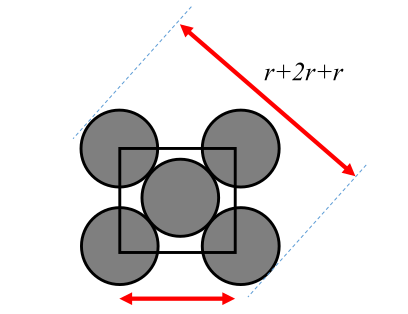
\includegraphics[width=0.7\textwidth]{images/cristallographie/cryst-005-000.png}
\caption{Schéma de réseau cristallin.}
\end{figure}

\begin{figure}[H]
\centering

\includegraphics[width=0.7\textwidth]{images/cristallographie/cryst-005-001.png}
\caption{Maille élémentaire et vecteurs de base.}
\end{figure}

\begin{figure}[H]
\centering
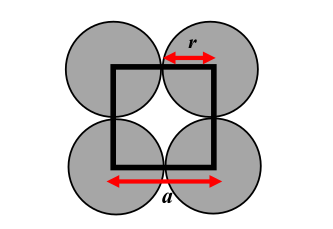
\includegraphics[width=0.7\textwidth]{images/cristallographie/cryst-006-002.png}
\caption{Structure cubique à faces centrées (CFC).}
\end{figure}

\begin{figure}[H]
\centering

\includegraphics[width=0.7\textwidth]{images/cristallographie/cryst-006-003.png}
\caption{Structure cubique centrée (CC).}
\end{figure}

\begin{figure}[H]
\centering
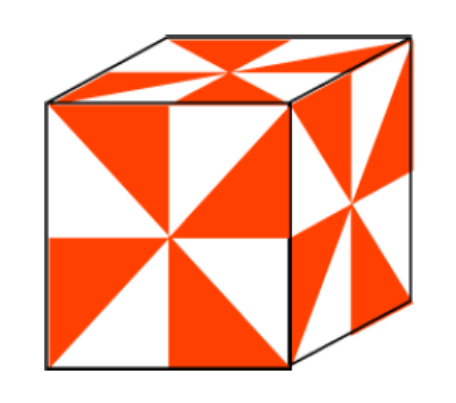
\includegraphics[width=0.7\textwidth]{images/cristallographie/cryst-010-004.png}
\caption{Indices de Miller d'un plan cristallin.}
\end{figure}

\begin{figure}[H]
\centering

\includegraphics[width=0.7\textwidth]{images/cristallographie/cryst-010-005.png}
\caption{Famille de plans réticulaires équivalents.}
\end{figure}

\begin{figure}[H]
\centering
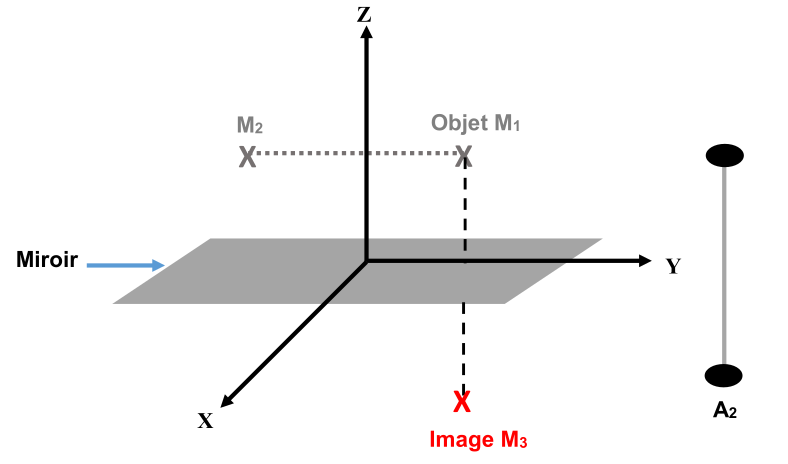
\includegraphics[width=0.7\textwidth]{images/cristallographie/cryst-011-006.png}
\caption{Loi de Bragg : diffraction des rayons X.}
\end{figure}

\begin{figure}[H]
\centering

\includegraphics[width=0.7\textwidth]{images/cristallographie/cryst-011-007.png}
\caption{Géométrie de la diffraction.}
\end{figure}

\begin{figure}[H]
\centering
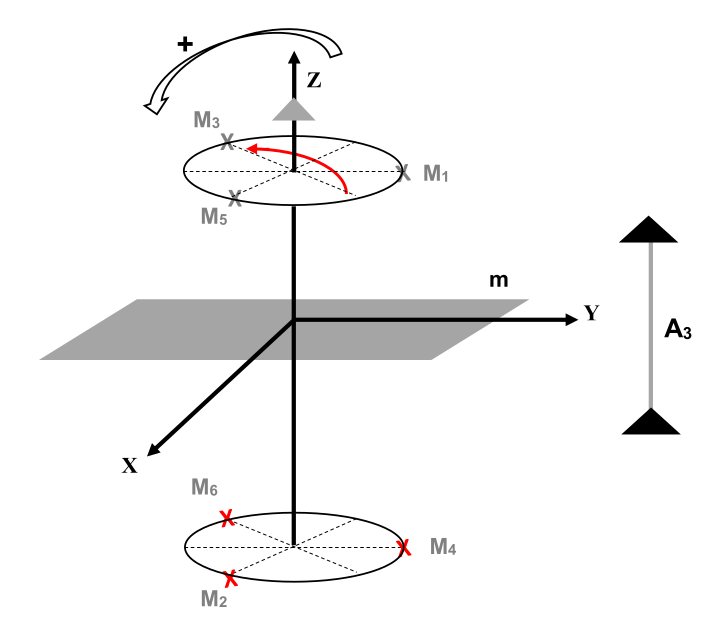
\includegraphics[width=0.7\textwidth]{images/cristallographie/cryst-012-008.png}
\caption{Réseau réciproque et vecteur de diffusion.}
\end{figure}

\begin{figure}[H]
\centering

\includegraphics[width=0.7\textwidth]{images/cristallographie/cryst-012-009.png}
\caption{Sphère d'Ewald et condition de diffraction.}
\end{figure}

\begin{figure}[H]
\centering
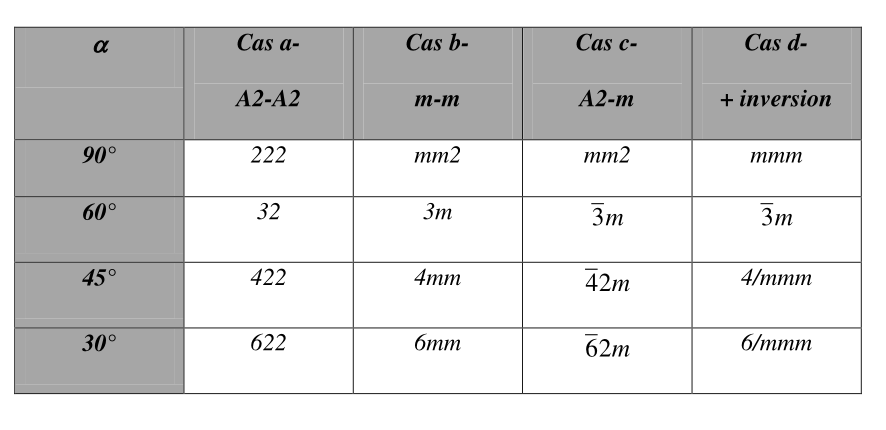
\includegraphics[width=0.7\textwidth]{images/cristallographie/cryst-013-010.png}
\caption{Structure NaCl : emboîtement de deux réseaux CFC.}
\end{figure}

\begin{figure}[H]
\centering

\includegraphics[width=0.7\textwidth]{images/cristallographie/cryst-013-011.png}
\caption{Sites interstitiels tétraédriques et octaédriques.}
\end{figure}

\begin{figure}[H]
\centering
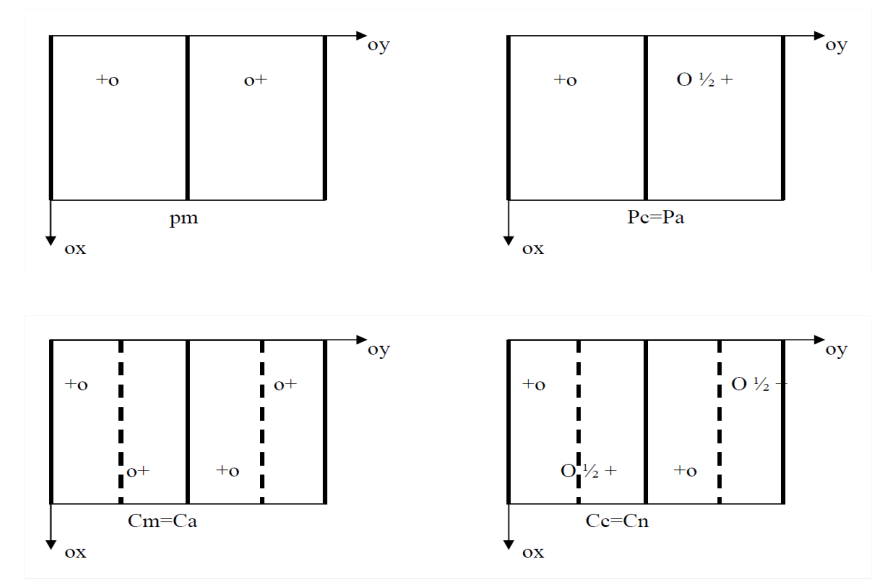
\includegraphics[width=0.7\textwidth]{images/cristallographie/cryst-014-012.png}
\caption{Structure hexagonale compacte (HC).}
\end{figure}

\begin{figure}[H]
\centering

\includegraphics[width=0.7\textwidth]{images/cristallographie/cryst-014-013.png}
\caption{Empilements compacts ABAB et ABCABC.}
\end{figure}

\ifdefined\inMainDoc\else\end{document}\fi
